\begin{center} \textbf{\huge Results} \end{center}
To evaluate the performance of our classification approaches we used the cumulative accuracy per interval and the cumulative accuracy over all points which. The batch/ offline method performs similar the first two test phase with but seams decreasing in the last interval.

 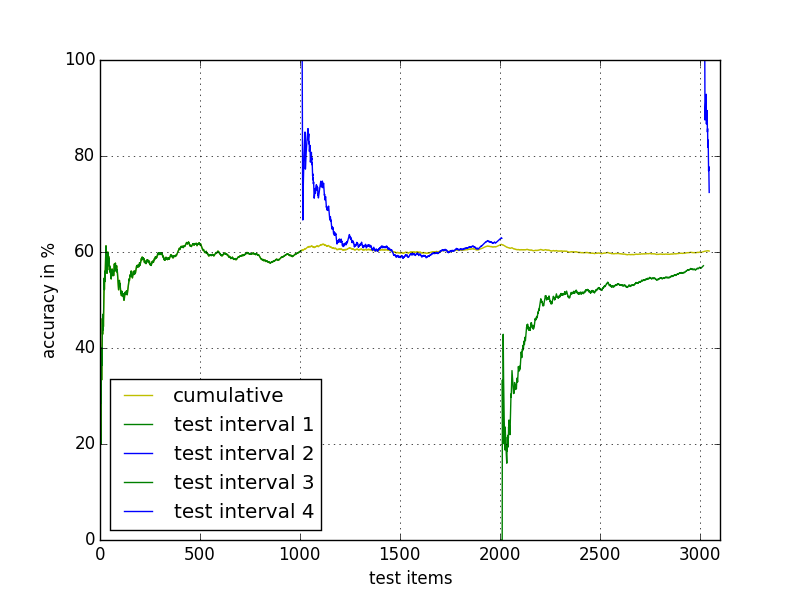
\includegraphics[width=0.2\textwidth]{./plots/batchPlot.png}\\

In the second scenario we applied the bruteforce model which rebuilt the model in the beginning of every interval.\\
   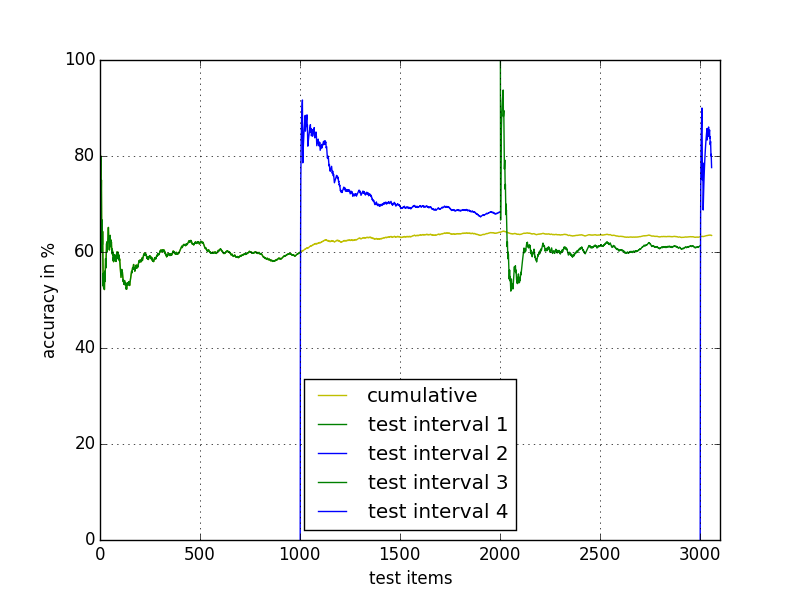
\includegraphics[width=0.2\textwidth]{./plots/bruteforce2_Plot.png}\\
In comparison with the batch version the bruteforce model gets higher accuracies in the intervals.\\

For the error-triggered model we set a threshold at 63\% of accuracy at which the model is recreated. After each model recreation, a sanity interval of 300 items takes place. In our experiments, we saw that the accuracy did not go below for a long time delaying the retraining period. Then two more retraining phases follow.\\
   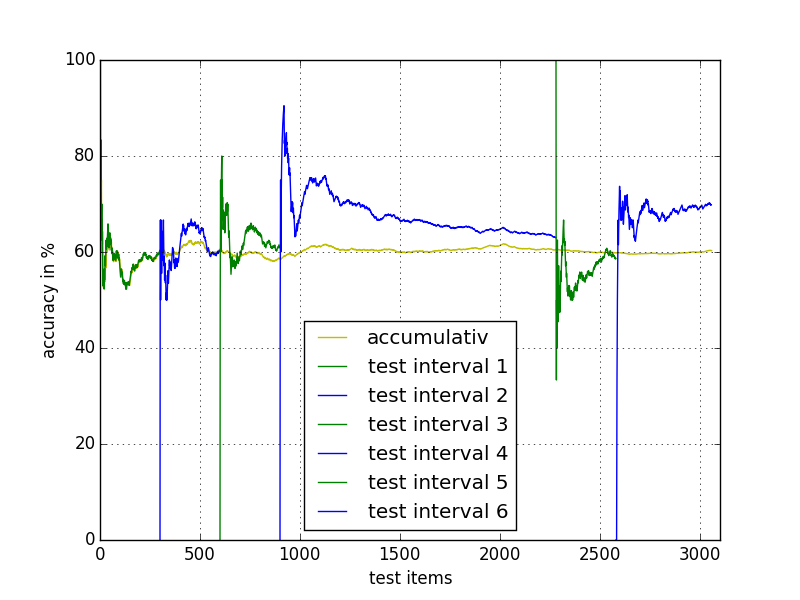
\includegraphics[width=0.2\textwidth]{./plots/errorTriggeredPlot}\\
In comparison to the batch update model, error-triggered has higher interval accuracy but due to the short retraining intervals, their accuracy results are similar on average. \\

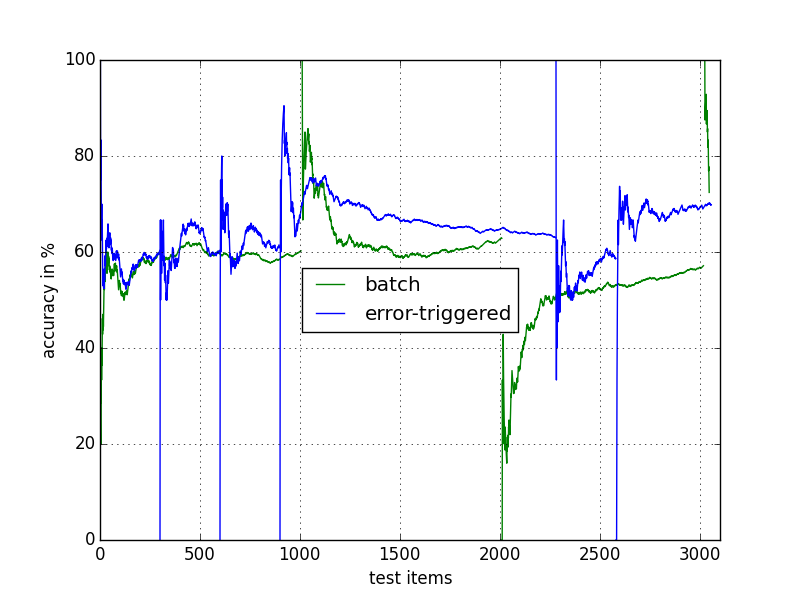
\includegraphics[width=0.2\textwidth]{./plots/errortriggered_batch}\\
Bruteforce and error-triggered methods have both higher interval accuracies in the test phases around the data points of 1000 and 2000. This might be caused by concept drift. 
\\

The incremental one clearly outperformed all the other model-update methods although the learning rate was mostly between 0.02 and 0 except for three peak times when it is around 0.6.

   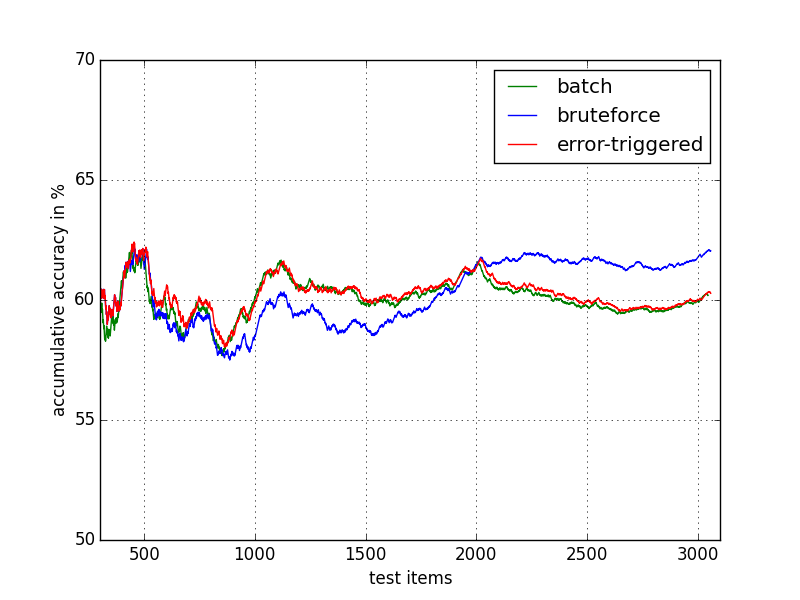
\includegraphics[width=0.2\textwidth]{./plots/allAccuracies}\\

